\chapter{Methodology}
\label{ch:methodology}

This chapter presents the core methodology of Cold Diffusion for \gls{ct} field-of-view extension in the sinogram domain~\cite{bansal2022cold}. We formulate truncation as a deterministic masking process, design the forward and reverse processes, and derive the training and sampling procedures.

\section{Problem Formulation}

\subsection{Truncation as Deterministic Masking}

We model \gls{ct} truncation as a progressive masking operation in the sinogram domain. Given a complete sinogram $\mathbf{x}_0 \in \mathbb{R}^{N_\theta \times N_t}$ where $N_\theta$ is the number of projection angles and $N_t$ is the number of detector elements, truncation removes information from the detector edges. This matches the deterministic degradation assumption of Cold Diffusion~\cite{bansal2022cold}.

Formally, we define a binary mask $\mathbf{M}_t \in \{0,1\}^{N_\theta \times N_t}$ at timestep $t \in \{0, 1, \ldots, T\}$ that indicates which detector elements are visible:
%
\begin{equation}
\mathbf{M}_t[i,j] = \begin{cases}
1 & \text{if detector column } j \text{ is kept at step } t \\
0 & \text{if detector column } j \text{ is masked (truncated) at step } t
\end{cases}
\end{equation}

The truncated sinogram at step $t$ is obtained by element-wise multiplication:
%
\begin{equation}
\mathbf{x}_t = \mathbf{x}_0 \odot \mathbf{M}_t
\label{eq:truncation_operation}
\end{equation}
%
where $\odot$ denotes element-wise multiplication.

\subsection{Progressive Masking Schedule}

To create a diffusion-like process, we design masks $\{\mathbf{M}_t\}_{t=0}^T$ that progressively truncate more of the sinogram. At timestep zero, $\mathbf{M}_0 = \mathbf{1}$ indicates no truncation with all detector elements visible. At the maximum timestep $T$, the mask $\mathbf{M}_T$ enforces maximum truncation with only $k_c$ center columns visible. For intermediate timesteps $0 < t < T$, the masks $\mathbf{M}_t$ represent intermediate truncation levels.

The parameter $k_c$ (keep\_center) controls the maximum truncation severity. For a sinogram with $N_t$ detector columns, the fully truncated state $\mathbf{x}_T$ preserves only the center $k_c$ columns.
In this thesis, truncation severity is primarily reported by $k_c$ because it directly corresponds to the preserved detector support. An equivalent ratio-based parameterization can also be used. If truncation ratio is defined as the total removed detector fraction, the mapping is \(k_c = (1-\rho)N_t\), where \(\rho\) is the truncation ratio.

\paragraph{Linear Masking Schedule} We adopt a linear schedule for the number of masked columns. At timestep $t$, we mask $n_t$ columns from each side:
%
\begin{equation}
n_t = \min\left\{ \left\lfloor \frac{N_t/2 \cdot (t+1)}{T} \right\rfloor, \max\_n \right\}
\label{eq:mask_schedule}
\end{equation}
%
where $\max\_n = \lfloor (N_t - k_c) / 2 \rfloor$ ensures we keep at least $k_c$ center columns.

The mask at timestep $t$ is:
%
\begin{equation}
\mathbf{M}_t[i,j] = \begin{cases}
1 & \text{if } n_t < j < N_t - n_t \\
0 & \text{otherwise}
\end{cases}
\end{equation}

The progressive masking schedule is shown in Figure~\ref{fig:progressive_masking_schedule}.

\begin{figure}[htbp]
\centering
\resizebox{\textwidth}{!}{%
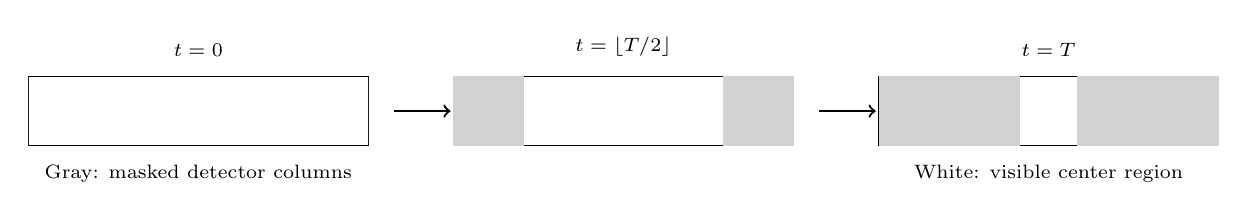
\begin{tikzpicture}[x=0.18cm,y=0.22cm,font=\scriptsize]
\newcommand{\drawstate}[3]{%
  \begin{scope}[shift={(#1,0)}]
    \pgfmathsetmacro{\rightedge}{24-#3}
    \draw (0,0) rectangle (24,4);
    \fill[gray!35] (0,0) rectangle (#3,4);
    \fill[gray!35] (\rightedge,0) rectangle (24,4);
    \node[above] at (12,4.6) {#2};
  \end{scope}
}
\drawstate{0}{$t=0$}{0}
\draw[->,thick] (25.8,2) -- (29.8,2);
\drawstate{30}{$t=\lfloor T/2 \rfloor$}{5}
\draw[->,thick] (55.8,2) -- (59.8,2);
\drawstate{60}{$t=T$}{10}
\node at (12,-1.6) {Gray: masked detector columns};
\node at (72,-1.6) {White: visible center region};
\end{tikzpicture}
}
\caption{Progressive masking in the forward process. As $t$ increases, edge detector columns are masked and the visible center region shrinks.}
\label{fig:progressive_masking_schedule}
\end{figure}

\section{Cold Diffusion Framework for Field-of-View Extension}

\subsection{Forward Process: Progressive Truncation}

The forward process deterministically degrades a clean sinogram $\mathbf{x}_0$ into increasingly truncated versions:
%
\begin{equation}
\mathcal{D}_t(\mathbf{x}_0) = \mathbf{x}_0 \odot \mathbf{M}_t = \mathbf{x}_t
\label{eq:forward_process}
\end{equation}

Unlike \gls{ddpm}, this is a \textit{deterministic} operation—there is no randomness. The same input $\mathbf{x}_0$ always produces the same $\mathbf{x}_t$ for a given $t$~\cite{ho2020denoising}.

\subsection{Reverse Process: Iterative Recovery}

The reverse process aims to recover the clean sinogram from a truncated version through iterative refinement. We train a neural network $f_\theta: \mathbb{R}^{N_\theta \times N_t} \times \mathbb{N} \to \mathbb{R}^{N_\theta \times N_t}$ that predicts the clean sinogram from a truncated input:
%
\begin{equation}
\hat{\mathbf{x}}_0 = f_\theta(\mathbf{x}_t, t)
\label{eq:network_prediction}
\end{equation}

The network $f_\theta$ is conditioned on the timestep $t$ to know the truncation level, allowing it to adapt its predictions accordingly.

To obtain the sinogram at the previous timestep $\mathbf{x}_{t-1}$, we apply the mask $\mathbf{M}_{t-1}$ to the predicted clean sinogram:
%
\begin{equation}
\mathbf{x}_{t-1} = \hat{\mathbf{x}}_0 \odot \mathbf{M}_{t-1}
\label{eq:reverse_step}
\end{equation}

In the executed inference pipeline, detector columns that are already observed in the truncated input are hard-replaced after each update to preserve measured data exactly. Let $\mathbf{x}_{\text{obs}}$ denote the input truncated sinogram and $\mathbf{M}_{\text{obs}}$ its binary visibility mask. The consistency projection is:
%
\begin{equation}
\mathbf{x}_{t-1} \leftarrow \mathbf{x}_{t-1} \odot (\mathbf{1} - \mathbf{M}_{\text{obs}}) + \mathbf{x}_{\text{obs}} \odot \mathbf{M}_{\text{obs}}
\label{eq:hard_replacement_observed}
\end{equation}
%
This step guarantees that physically measured detector values remain unchanged throughout reverse sampling.

\subsection{Reverse-Update and Sampling Strategies}
\label{sec:sampling_strategies}

The original Cold Diffusion paper describes two reverse-update views that are directly relevant here~\cite{bansal2022cold}. In the first view, corresponding to Algorithm 1, the model predicts a clean estimate at each step and directly projects that estimate to the next state through the degradation operator at step $t-1$. Under truncation masking, this behavior is equivalent to Equation~\ref{eq:reverse_step}, where the previous iterate is reconstructed from the latest clean prediction and the next mask. In the second view, corresponding to Algorithm 2, the update is written in residual form. The state at $t-1$ is obtained by taking the current state at $t$ and adding only the newly required correction between two consecutive degradation levels.

For field-of-view extension under truncation, this residual form becomes:

\begin{equation}
\mathbf{x}_{t-1} = \mathbf{x}_t + (\hat{\mathbf{x}}_0 - \mathbf{x}_t) \odot (\mathbf{M}_{t-1} - \mathbf{M}_t)
\label{eq:algo2_residual_update}
\end{equation}

Here, $(\mathbf{M}_{t-1} - \mathbf{M}_t)$ identifies newly unmasked regions, and only those regions are updated using the current clean estimate. The already available region is carried forward from $\mathbf{x}_t$ instead of being overwritten at every step. This is the practical difference between Algorithm 1 style direct replacement and Algorithm 2 style residual correction. In our setting, where truncation boundaries are progressively revealed, residual correction provides a better bias toward consistency across steps and helps reduce the accumulation of boundary errors.

\begin{algorithm}[htbp]
\caption{Algorithm 1 Style Reverse Update (Direct Replacement)}
\label{alg:algo1_update}
\begin{algorithmic}[1]
\REQUIRE Current state $\mathbf{x}_t$, timestep $t$, network $f_\theta$, next mask $\mathbf{M}_{t-1}$
\ENSURE Updated state $\mathbf{x}_{t-1}$
\STATE $\hat{\mathbf{x}}_0 \gets f_\theta(\mathbf{x}_t, t)$
\STATE $\mathbf{x}_{t-1} \gets \hat{\mathbf{x}}_0 \odot \mathbf{M}_{t-1}$
\STATE \textbf{return} $\mathbf{x}_{t-1}$
\end{algorithmic}
\end{algorithm}

\begin{algorithm}[htbp]
\caption{Algorithm 2 Style Reverse Update (Residual Correction)}
\label{alg:algo2_update}
\begin{algorithmic}[1]
\REQUIRE Current state $\mathbf{x}_t$, timestep $t$, network $f_\theta$, masks $\mathbf{M}_{t}, \mathbf{M}_{t-1}$
\ENSURE Updated state $\mathbf{x}_{t-1}$
\STATE $\hat{\mathbf{x}}_0 \gets f_\theta(\mathbf{x}_t, t)$
\STATE $\mathbf{x}_{t-1} \gets \mathbf{x}_t + (\hat{\mathbf{x}}_0 - \mathbf{x}_t) \odot (\mathbf{M}_{t-1} - \mathbf{M}_t)$
\STATE \textbf{return} $\mathbf{x}_{t-1}$
\end{algorithmic}
\end{algorithm}

For reproducibility, all experiments and results reported in this thesis use Algorithm 2 for inference. Algorithm 1 is included as a methodological reference and conceptual comparison, but it is not used as the reporting-time sampling rule in the executed evaluation pipeline.

At inference time, given a truncated sinogram $\mathbf{x}_T$, we iteratively recover the complete sinogram by running the reverse process from $t=T$ to $t=0$. The update operator in each step is chosen according to the Algorithm 1 or Algorithm 2 view described above. Algorithm~\ref{alg:sampling} summarizes this generic procedure without repeating both branches in detail.

\begin{algorithm}[htbp]
\caption{Cold Diffusion Sampling for Field-of-View Extension}
\label{alg:sampling}
\begin{algorithmic}[1]
\REQUIRE Truncated sinogram $\mathbf{x}_T$, trained network $f_\theta$, masks $\{\mathbf{M}_t\}_{t=0}^T$, update rule $\mathcal{U}$ (Algorithm 1 or Algorithm 2 style)
\ENSURE Recovered sinogram $\hat{\mathbf{x}}_0$
\FOR{$t = T$ \textbf{to} $1$}
    \STATE $\hat{\mathbf{x}}_0 \gets f_\theta(\mathbf{x}_t, t)$ \hfill // Predict clean sinogram
    \STATE $\mathbf{x}_{t-1} \gets \mathcal{U}(\mathbf{x}_t, \hat{\mathbf{x}}_0, \mathbf{M}_{t}, \mathbf{M}_{t-1})$
\ENDFOR
\STATE \textbf{return} $\hat{\mathbf{x}}_0$ \hfill // Final prediction from the last iteration
\end{algorithmic}
\end{algorithm}

For completeness, we also summarize the training loop that is paired with the above reverse-sampling design in the executed experiments.

\begin{algorithm}[htbp]
\caption{Training Cold Diffusion for Field-of-View Extension}
\label{alg:training}
\begin{algorithmic}[1]
\REQUIRE Training data $\mathcal{D}_{\text{train}} = \{\mathbf{x}_0^{(i)}\}_{i=1}^N$, timesteps $T$, masks $\{\mathbf{M}_t\}_{t=1}^T$
\ENSURE Trained network parameters $\theta$
\STATE Initialize network $f_\theta$ with random weights
\WHILE{training budget not exhausted}
    \STATE Sample minibatch $\{\mathbf{x}_0^{(i)}\}_{i=1}^B$ from $\mathcal{D}_{\text{train}}$
    \FOR{each $\mathbf{x}_0^{(i)}$ in minibatch}
        \STATE Sample $t^{(i)} \sim \text{Uniform}(1, T)$
        \STATE Compute $\mathbf{x}_t^{(i)} = \mathbf{x}_0^{(i)} \odot \mathbf{M}_{t^{(i)}}$
        \STATE Predict $\hat{\mathbf{x}}_0^{(i)} = f_\theta(\mathbf{x}_t^{(i)}, t^{(i)})$
        \STATE Compute $\mathcal{L}^{(i)} = \| \hat{\mathbf{x}}_0^{(i)} - \mathbf{x}_0^{(i)} \|_1$
    \ENDFOR
    \STATE $\mathcal{L}_{\text{batch}} = \frac{1}{B} \sum_{i=1}^B \mathcal{L}^{(i)}$
    \STATE Update $\theta$ using gradient descent: $\theta \gets \theta - \eta \nabla_\theta \mathcal{L}_{\text{batch}}$
\ENDWHILE
\STATE \textit{Practical note:} the executed experiments use a fixed-step training design rather than adaptive convergence stopping.
\end{algorithmic}
\end{algorithm}

\subsection{Role of Classical Extrapolation References}

In the executed pipeline, classical extrapolation (WCE) is included as an explicit reference branch in evaluation to provide a physics-based non-learned comparator. Let $\mathcal{E}_{\text{WCE}}$ denote the extrapolation operator applied to a truncated sinogram $\mathbf{x}_t$:
\begin{equation}
\mathbf{x}^{\text{ref}}_t = \mathcal{E}_{\text{WCE}}(\mathbf{x}_t).
\end{equation}
This reference is reported alongside learned methods to contextualize gains and failure modes. For model training, the input remains the truncated sinogram itself rather than a WCE-preprocessed variant. This design avoids injecting method-specific extrapolation bias into the learning target, keeps the degradation model aligned with the physical truncation process, and allows baseline comparisons to attribute improvements to the learned model rather than to a fixed analytical prefill step. At the same time, using WCE-derived inputs as auxiliary conditioning remains a valid extension for future study and can be evaluated separately under controlled protocols.

\section{Training}

\subsection{Training Objective}

We train the network to minimize the $L_1$ (or $L_2$) distance between the predicted and ground truth sinograms:
%
\begin{equation}
\mathcal{L} = \mathbb{E}_{\mathbf{x}_0, t} \left[ \| f_\theta(\mathcal{D}_t(\mathbf{x}_0), t) - \mathbf{x}_0 \|_1 \right]
\label{eq:training_loss}
\end{equation}

For each training iteration, we sample a clean sinogram and a random timestep, apply the corresponding mask to obtain a truncated input, and minimize the $L_1$ distance between the network's prediction and the ground truth, as detailed in Algorithm~\ref{alg:training}. $L_1$ loss is used by default as it tends to produce sharper reconstructions than $L_2$ loss.

\subsection{Exponential Moving Average (EMA)}

We maintain an \gls{ema} of model parameters during training:
%
\begin{equation}
\theta_{\text{EMA}} \gets \beta \cdot \theta_{\text{EMA}} + (1 - \beta) \cdot \theta
\end{equation}
%
with $\beta = 0.9995$. The \gls{ema} model typically produces smoother and more stable predictions, especially for generative tasks. We use the \gls{ema} weights for evaluation and inference.

\subsection{Learning Rate Scheduling}

We employ a cosine annealing learning rate schedule with optional warmup:
%
\begin{equation}
\eta(s) = \begin{cases}
\eta_0 \cdot \frac{s}{s_{\text{warmup}}} & \text{if } s < s_{\text{warmup}} \\
\eta_{\text{min}} + \frac{1}{2}(\eta_0 - \eta_{\text{min}})\left(1 + \cos\left(\frac{s - s_{\text{warmup}}}{s_{\text{total}} - s_{\text{warmup}}} \pi\right)\right) & \text{otherwise}
\end{cases}
\label{eq:lr_schedule}
\end{equation}
%
where $s$ is the current step, $\eta_0$ is the initial learning rate, $\eta_{\text{min}}$ is the minimum learning rate, $s_{\text{warmup}}$ is the warmup period, and $s_{\text{total}}$ is the total training steps.

\subsection{Mixed Precision Training}

To accelerate training and reduce memory consumption, we use \gls{amp} with PyTorch's \texttt{torch.cuda.amp}. Computationally intensive operations (convolutions, matrix multiplications) are performed in \texttt{float16}, while numerically sensitive operations (loss computation, batch normalization) remain in \texttt{float32}.

\section{Network Architecture}

\subsection{U-Net Backbone}

We adopt a U-Net architecture~\cite{ronneberger2015unet} as the backbone of $f_\theta$. Figure~\ref{fig:method_unet_architecture} provides an overview of the encoder-decoder structure and the main components at each level.

\begin{figure}[htbp]
\centering
\resizebox{\textwidth}{!}{%
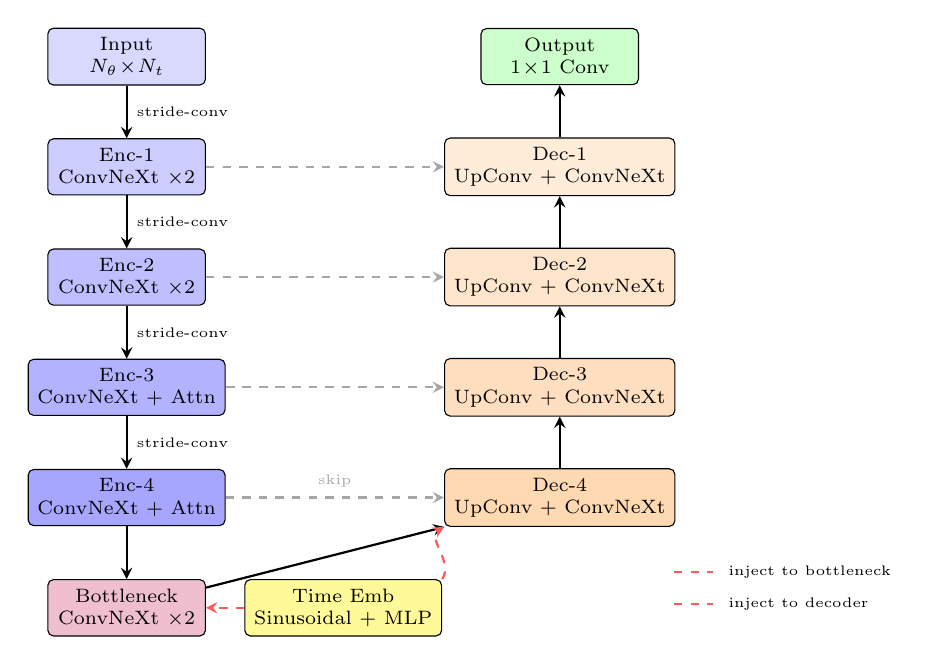
\begin{tikzpicture}[
  box/.style={draw, rounded corners=2pt, minimum width=2.0cm, minimum height=0.55cm,
               font=\scriptsize, align=center, fill=#1},
  arr/.style={->, thick, >=stealth},
  skip/.style={->, thick, >=stealth, dashed, gray!70},
  font=\scriptsize
]

% ---- encoder column (left) ----
\node[box=blue!15]   (in)   at (0,0)   {Input\\$N_\theta\!\times\!N_t$};
\node[box=blue!20]   (e1)   at (0,-1.4) {Enc-1\\ConvNeXt $\times$2};
\node[box=blue!25]   (e2)   at (0,-2.8) {Enc-2\\ConvNeXt $\times$2};
\node[box=blue!30]   (e3)   at (0,-4.2) {Enc-3\\ConvNeXt $+$ Attn};
\node[box=blue!35]   (e4)   at (0,-5.6) {Enc-4\\ConvNeXt $+$ Attn};

% ---- bottleneck ----
\node[box=purple!25] (bn)   at (0,-7.0) {Bottleneck\\ConvNeXt $\times$2};

% ---- decoder column (right) ----
\node[box=orange!30] (d4)   at (5.5,-5.6) {Dec-4\\UpConv $+$ ConvNeXt};
\node[box=orange!25] (d3)   at (5.5,-4.2) {Dec-3\\UpConv $+$ ConvNeXt};
\node[box=orange!20] (d2)   at (5.5,-2.8) {Dec-2\\UpConv $+$ ConvNeXt};
\node[box=orange!15] (d1)   at (5.5,-1.4) {Dec-1\\UpConv $+$ ConvNeXt};
\node[box=green!20]  (out)  at (5.5,0)    {Output\\$1\!\times\!1$ Conv};

% ---- timestep embedding (right of bottleneck) ----
\node[box=yellow!40] (temb) at (2.75,-7.0) {Time Emb\\Sinusoidal $+$ MLP};

% ---- encoder downward arrows ----
\draw[arr] (in) -- node[right,font=\tiny]{stride-conv} (e1);
\draw[arr] (e1) -- node[right,font=\tiny]{stride-conv} (e2);
\draw[arr] (e2) -- node[right,font=\tiny]{stride-conv} (e3);
\draw[arr] (e3) -- node[right,font=\tiny]{stride-conv} (e4);
\draw[arr] (e4) -- (bn);

% ---- decoder upward arrows ----
\draw[arr] (bn) -- (d4);
\draw[arr] (d4) -- (d3);
\draw[arr] (d3) -- (d2);
\draw[arr] (d2) -- (d1);
\draw[arr] (d1) -- (out);

% ---- skip connections ----
\draw[skip] (e4.east) -- node[above,font=\tiny]{skip} (d4.west);
\draw[skip] (e3.east) to[out=0,in=180] (d3.west);
\draw[skip] (e2.east) to[out=0,in=180] (d2.west);
\draw[skip] (e1.east) to[out=0,in=180] (d1.west);

% ---- time embedding injection (two branches; labels moved to legend) ----
\draw[arr,dashed,red!65] (temb.west) -- (bn.east);
\draw[arr,dashed,red!65] (temb.north east) to[out=55,in=-150] (d4.south west);

% ---- legend (avoids overlap with flow boxes) ----
\draw[red!65,dashed,thick] (6.95,-6.55) -- (7.45,-6.55);
\node[anchor=west,font=\tiny] at (7.52,-6.55) {inject to bottleneck};
\draw[red!65,dashed,thick] (6.95,-6.95) -- (7.45,-6.95);
\node[anchor=west,font=\tiny] at (7.52,-6.95) {inject to decoder};

\end{tikzpicture}
}
\caption{Overview of the time-conditioned U-Net architecture used in this work. The encoder progressively downsamples the sinogram through four levels of ConvNeXt blocks, with linear attention applied in the deeper encoder levels. Skip connections pass encoder feature maps directly to the corresponding decoder levels. A sinusoidal timestep embedding is projected by an MLP and injected at the bottleneck and decoder stages to condition the network on the current truncation level.}
\label{fig:method_unet_architecture}
\end{figure}

U-Net is well-suited for sinogram processing due to its multi-scale feature extraction capability where the encoder captures both local and global context, its skip connections that preserve fine details lost during downsampling, and its symmetric design that enables efficient information flow from input to output.

Our U-Net consists of an encoder with 4 downsampling blocks (each containing ConvNeXt-style blocks with depthwise convolution and \gls{gelu} activation~\cite{liu2022convnet}, with linear attention in the deeper encoder levels, and downsampling via strided convolution), a bottleneck with additional ConvNeXt blocks at the lowest resolution, a decoder with 4 upsampling blocks (each containing upsampling via transposed convolution, concatenation with encoder features through skip connections, and ConvNeXt blocks), and an output head using $1 \times 1$ convolution to produce single-channel sinogram predictions.

\subsection{Timestep Conditioning}

To condition the network on timestep $t$, we use sinusoidal position embeddings~\cite{vaswani2017attention}:
%
\begin{align}
\text{emb}(t, 2i) &= \sin\left(\frac{t}{10000^{2i/d}}\right) \\
\text{emb}(t, 2i+1) &= \cos\left(\frac{t}{10000^{2i/d}}\right)
\end{align}
%
where $d$ is the embedding dimension. The embedding is passed through an \gls{mlp} and added to feature maps at each resolution level.

\subsection{ConvNeXt Blocks}

We use ConvNeXt blocks~\cite{liu2022convnet}, a modernized version of residual blocks:

\begin{equation}
\begin{split}
\mathbf{y} &= \text{DWConv}_{7\times7}(\mathbf{x}) \\
\mathbf{y} &= \text{GroupNorm}(\mathbf{y}) \\
\mathbf{y} &= \text{Conv}_{3\times3}(\mathbf{y}) \cdot m \\
\mathbf{y} &= \text{GELU}(\mathbf{y}) \\
\mathbf{y} &= \text{Conv}_{3\times3}(\mathbf{y}) \\
\text{output} &= \mathbf{x} + \mathbf{y}
\end{split}
\end{equation}

In our implementation, the ConvNeXt-style block follows the same depthwise-plus-pointwise design principle but uses GroupNorm and $3\times3$ expansion/compression convolutions as a practical variant for stable sinogram training.

\subsection{Attention Mechanism}

At lower resolutions, we incorporate lightweight linear attention to capture long-range dependencies in the sinogram, inspired by attention mechanisms in transformers~\cite{vaswani2017attention}. This is particularly useful as truncated regions may require information from distant non-truncated areas.

\section{Design Choices and Rationale}

\subsection{Rationale for Cold Diffusion and Projection-Domain Modeling}

Cold Diffusion is selected because truncation is a deterministic masking process rather than a stochastic noising process. This alignment keeps the degradation model close to the acquisition mechanism and gives each timestep a clear physical meaning in terms of visible detector support. The truncated sinogram itself already provides structured context, so the model can exploit available projection information directly while adapting to timestep-dependent truncation severity.

Working in the sinogram domain follows the same principle. Truncation is introduced in projection space, so recovery at this stage avoids learning artifact compensation only after nonlinear reconstruction effects have appeared in image space. This design also avoids additional forward-projection loops during training and keeps the restored sinogram compatible with downstream reconstruction operators.

\subsection{Rationale for Iterative Refinement}

Single-step predictors must infer the entire missing region in one pass, which is difficult when truncation is severe. The iterative reverse process instead decomposes recovery into multiple stages, where coarse structure is formed first and refined progressively. This staged behavior improves stability at truncation boundaries and allows correction of intermediate errors across timesteps.

\section{Summary}

This chapter presented the core methodology, including the formulation of \gls{ct} truncation as progressive deterministic masking, the Cold Diffusion framework adapted for sinogram recovery, the forward process implementing progressive truncation and reverse process enabling iterative recovery, the training procedure utilizing $L_1$ loss and \gls{ema}, and the U-Net architecture with timestep conditioning. The next chapter details the experimental design and evaluation protocols used to analyze these choices.
